
\section{Medium access}

Control medium access, but allow concurrent medium usage $\Rightarrow$
multiplexing.

\begin{table}[!h]
    \begin{tabular}{|r|cccc|}
        \hline
        & SDMA & FDMA & TDMA & CDMA \\
        \hline
        Coordination & None & Frequency assignment & Time synchronization & Code coordinations \\
        Viable & x & x & v & v \\
        \hline
    \end{tabular}
\end{table}

\begin{itemize}
    \item \textbf{Space Division Multiple Access (SDMA)}: divide space
        so that devices do not interfere.
        \begin{center}
            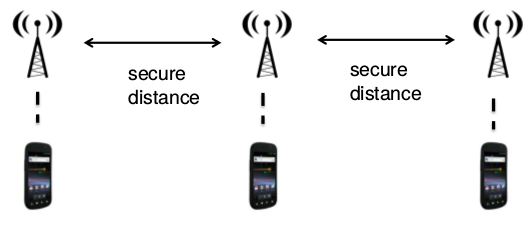
\includegraphics[width=0.6\linewidth]{img/SDMA.png}
        \end{center}

        \begin{itemize}
            \item Simple, but pure SDMA require huge secure distance and one
                station per end point: not viable in practice without other
                multiplex methods!
        \end{itemize}

    \item \textbf{Frequency Division Multiple Access (FDMA)}:
        Frequencies permanently assigned to transmission channels
        \begin{center}
            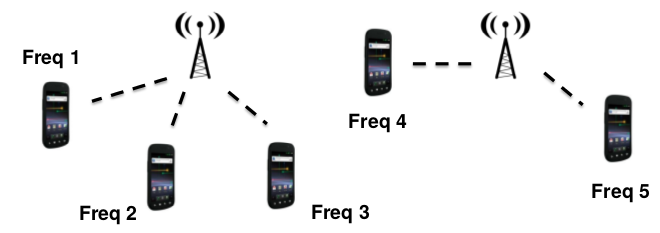
\includegraphics[width=0.6\linewidth]{img/FDMA.png}
        \end{center}

        \begin{itemize}
            \item One frequency per station and these frequency require
                \textit{guard-bands} between them such that they are more robust
                against interferences
        \end{itemize}
        \begin{center}
            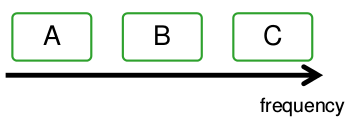
\includegraphics[width=0.3\linewidth]{img/guard.png}
        \end{center}

    \item \textbf{Time Division Multiple Access (TDMA)}:
        Time is divided into slots and only one station per slot can
        access medium
        \begin{center}
            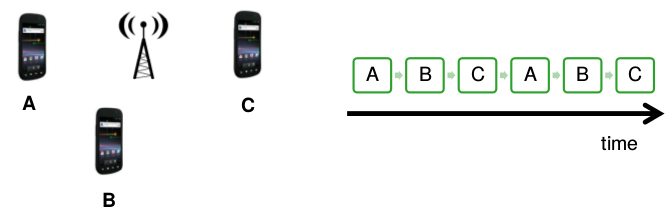
\includegraphics[width=0.6\linewidth]{img/TDMA.png}
        \end{center}

        \begin{itemize}
            \item One frequency, time division can be done in
                control software 
            \item but $\Rightarrow$ Require \textbf{exact timing} between stations
                (use \textit{guard-times} between slots to be more tolerant
                against timing variations)
        \end{itemize}

    \item \textbf{Code Division Multiple Access (CDMA)}: Each sender
        uses a different code that is applied to the data stream and if
        receiver know the code it can decode the data.

        \begin{enumerate}
            \item Sender A: \begin{tabular}{l} send bit=1\\
                Code=010011\\ Ouput = (-1 +1 -1 -1 +1 +1)\end{tabular}
            \item Sender B: \begin{tabular}{l} send bit=0\\
                Code=110101\\ Ouput = (-1 -1 +1 -1 +1 -1)\end{tabular}
            \item superimposed: (-2 0 0 -2 +2 0)
            \item Extract A: (-2 0 0 -2 +2 0) * (-1 +1 -1 -1 +1 +1) = 6
                $\geq$ 0 $\Rightarrow$ original bit is 1
        \end{enumerate}

        \begin{itemize}
            \item Need much longer codes which needs more bandwidth than
                original. 
            \item Coordination between station to have different code or
                stations choose code randomly
            \item Senders have to adapt their transmission power to all have
                the same strength at a receiver
        \end{itemize}
\end{itemize}

\subsection{Assignment}

Instead of have a central manager who assigns resources which can leads
to a waste of resources if node doest not want to send:
\begin{itemize}
    \item \textbf{Demand-based assignment}
        \begin{itemize}
            \item \textit{Polling}: Ask is node has something to
                transmit, if not ask next node.

                $\Rightarrow$ Overhead and not scalable + need
                central coordination

            \item \textit{Token-passing}: token is a special signal
                or packet

                $\Rightarrow$ Need to know next node + token
                regeneration if it is loss + what about fairness if
                node keep token for long time
        \end{itemize}

    \item \textbf{Random access}: Sends when it wants with
        collisions possibilities.

        $\Rightarrow$ Fully distributed without coordinator
        but collisions increases with number of nodes and
        traffic load
\end{itemize}


\subsection{ALOHAnet}
\begin{itemize}
    \item All node send packets/frame of identical duration $T$ on a single
        channel ($\rightarrow$ TDMA)

    \item Collisions possible if two node sends a packet at same time,
        to avoid this:
        \begin{enumerate}
            \item Sender sends a packet
            \item Collision happens
            \item Receiver receives a garbled packet
                \begin{itemize}
                    \item Receiver does not send ACK to sender
                    \item Sender knows that collision has happened
                \end{itemize}
            \item Sender waits a random time in the range [0,...,B] (“backoff period”)
            \item Send tries again (-> Step 1)
        \end{enumerate}

    \item Use time slots to limited collision to one timeslots (require
        synchronized clock on all nodes)

    \item Carrier-Sense Multiple Access (CSMA): node listen for a free
        channel before sending (if busy, wait for a random time)

        $\Rightarrow$ Still collision because of propagation delay

    \item CSMA with Collision Detection (CSMA/CD): node listening while
        sending in order to detect collision at receiver (need complex
        hardware)

        $\Rightarrow$ No loss time to send end of frame when collision
        detected

    \item CSMA/CA: 
        \begin{itemize}
            \item If channel free 
                \begin{enumerate}
                    \item Node wait for channel stay free for the IFS time
                        (Inter-Frame Spacing)
                    \item Node sends
                \end{enumerate}
            \item If channel is in use 
                \begin{enumerate} 
                    \item Node waits until current transmission is over
                    \item Node waits for channel to stay free for the IFS time
                    \item Node waits additional random backoff time
                \end{enumerate}
        \end{itemize}

        \begin{center}
            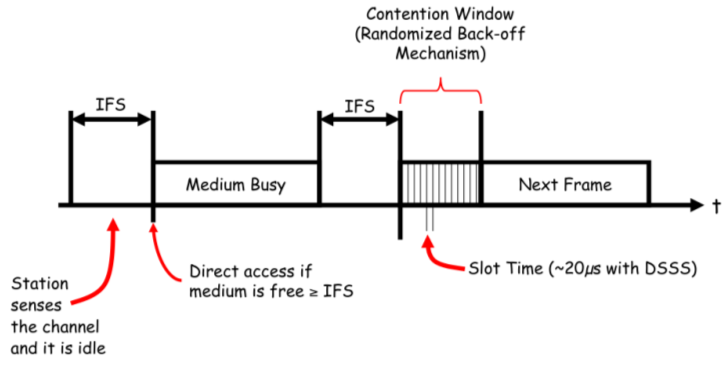
\includegraphics[width=0.7\linewidth]{img/CSMA.png}
        \end{center}

    \item CSMA/CA with ACK: ACK frames are given higher priority than
        normal data frames $\Rightarrow$ Receiver wait Shorter IFS
        (SIFS < IFS) before sending

    \item CSMA/CA with RTS/CTS: solve the \textit{hidden station
        problem} (CSMA/CA and CSMA/CD are still unreliable with this
        problem)
        \begin{enumerate}
            \item Before sending data, node A sends RTS (Request to
                Send) control frame to node B after medium was
                free for IFS time
            \item  Node B sends CTS (Clear to Send) to node A after
                medium was free for SIFS time
            \item Node C also hears the CTS frame -> node C waits
            \item Node A can send now
        \end{enumerate}

        $\Rightarrow$ Collision still possible for RTS, CTS packet which has
        a small impact as these control frame packet are smaller.
\end{itemize}


